\documentclass[tikz,border=5pt]{standalone}
\usepackage{newtxmath}
\begin{document}
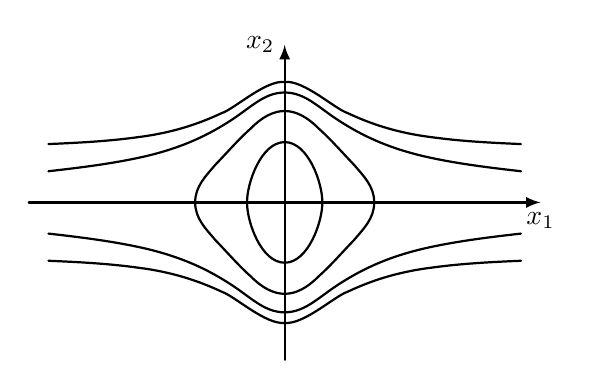
\begin{tikzpicture}[
    line cap=round,line join=round,thick,
    phase/.pic={
        \draw[draw=black] (-3,0.741)
        .. controls (-2.503,0.762) and (-2.186,0.784) .. (-1.854,0.83)
        .. controls (-1.428,0.884) and (-1.093,0.996) .. (-0.798,1.135)
        .. controls (-0.639,1.187) and (-0.241,1.556) .. (0,1.53);
        \draw[draw=black] (-3,0.396)
        .. controls (-2.586,0.443) and (-2.169,0.494) .. (-1.768,0.586)
        .. controls (-1.344,0.686) and (-1.029,0.824) .. (-0.732,1.011)
        .. controls (-0.446,1.185) and (-0.275,1.395) .. (0,1.396);
        \draw[draw=black] (-1.137,0)
        .. controls (-1.137,0.207) and (-1,0.336) .. (-0.879,0.48)
        .. controls (-0.73,0.633) and (-0.593,0.795) .. (-0.431,0.939)
        .. controls (-0.291,1.082) and (-0.144,1.161) .. (0.00,1.161);
        \draw[draw=black] (-0.478,0)
        .. controls (-0.481,0.243) and (-0.299,0.766) .. (0,0.766);
    }
]
    \draw[-latex] (-3.25,0) -- (3.25,0) node[below] {$x_1$};
    \draw[-latex] (0,-2) -- (0,2) node[left] {$x_2$};
    \path 
        pic {phase} 
        pic[xscale=-1] {phase} 
        pic[yscale=-1] {phase} 
        pic[scale=-1] {phase}
    ;
\end{tikzpicture}
\end{document}